\clearpage
\twocolumn
\section{Attention and Feature Responses during Action Generation}
\label{sec:supp-attention-analysis}
\label{sec:attention}
How do visual perturbations show up in the attention computations of $\pi_{0.5}$ during action generation? Changing the main camera alters deep features at the positions of the unchanged wrist image. At L18, clean--perturbed differences in attention weights shrink from the first to the last sampled generation step, while differences in attention output grow, in all four family means. This is an additional study, beside the restoration test of main Sec.~\ref{M-sec:restoration}; the main paper mentions it once, in Related Work, and does not rely on it.

Attention outputs depend on both the attention weights and the norms of the transformed value vectors~\cite{kobayashi2020}, so a change in the weights must be read together with the features being combined. We first examine the content available to attention, then how it is weighted and transformed as the plan is refined.

\subsection{Visual Changes Reach beyond the Altered View}
Changing the main camera changes deep features at unchanged wrist-image positions. In a 36-task LIBERO study, we rotate the main camera by $15^\circ$ while keeping the physical state, wrist image, and language instruction fixed. We examine the wrist-image \emph{value vectors} ($V$): the feature content that attention reads and combines. These vectors are unchanged at L1 but change at L9 and L18 (Sec.~\ref{supp:legacy-attention}). A deep feature at a wrist-image position thus carries context from the main view, even when the wrist pixels are identical.

Which layer redistributes wrist attention more depends on whether the wrist's share of attention is counted. In the same study, we normalize the wrist probabilities to sum to one and measure their change by conditional total variation (TV), half the sum of absolute probability differences. Weighting each comparison by the mean total wrist attention of the clean and perturbed runs puts this redistribution on the scale of all attention. At generation step 0 under baseline lighting, L18 has the larger conditional TV, but L9 has the larger mass-weighted TV (Table~\ref{tab:attention-context}a), in all 36 tasks.

The matched LIBERO-Plus recordings show the same depth pattern under Camera and Sensor Noise: mean wrist-value responses are zero at L1 and nonzero at L9 and L18 (Table~\ref{tab:attention-context}b), on the 28 common tasks. These values are cached once per observation, and the action expert attends to them at every generation step.

\begin{table}[t]
\centering\small
\setlength{\tabcolsep}{5pt}
\textbf{(a) LIBERO: wrist-attention redistribution}\\[2pt]
\begin{tabular}{@{}lrr@{}}
\toprule
Wrist-attention change & L9 & L18\\\midrule
Within-wrist TV (\%) & 15.75 & \textbf{25.18}\\
Mass-weighted TV (pp) & \textbf{5.45} & 2.33\\\bottomrule
\end{tabular}
\vspace{5pt}

\textbf{(b) LIBERO-Plus: wrist-value responses}\\[2pt]
\begin{tabular}{@{}lrrr@{}}
\toprule
Perturbation & L1 & L9 & L18\\\midrule
Camera & 0 & 0.514 & 0.275\\
Sensor Noise & 0 & 0.415 & 0.232\\\bottomrule
\end{tabular}
\caption{\textbf{Counting the wrist's share of attention reverses the layer ranking; wrist features respond at depth.} (a) Fixed-state LIBERO study: main-camera $0^\circ\!\rightarrow15^\circ$, baseline lighting, generation step 0, 36 tasks. Each conditional TV is weighted by its mean clean/perturbed wrist-attention mass before task-equal averaging; the layer ordering reverses in every task. (b) First-query wrist-value differences relative to the clean wrist-value norm, using the Camera (102 pairs) and Sensor Noise (110 pairs) subsets of the matched LIBERO-Plus panel, each on 28 tasks. Entries are task-equal means. Normalized probabilities use \%; mass-weighted changes use percentage points (pp). Full measures and value-response intervals: Secs.~\ref{sec:supp-plus-joint-readout} and~\ref{supp:legacy-attention}.}
\label{tab:attention-context}
\end{table}

\subsection{Attention-Weight Differences Shrink while Output Differences Grow}
\begin{figure*}[t]
\centering
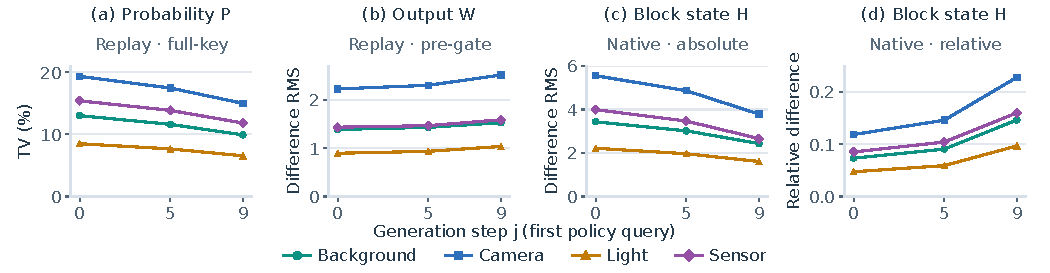
\includegraphics[width=\textwidth]{revised_figures/figure5_attention.pdf}
\caption{\textbf{Attention-weight differences shrink while output-feature differences grow.} At L18, (a) full-key probability TV decreases from the first to the last sampled generation step, while (b) the raw RMS difference in the projected attention output increases. Both are recomputed at each run's saved generation states. The block-end state recorded during the policy's own generation has (c) decreasing absolute differences but (d) increasing differences relative to the shrinking clean state. All panels use the same 404 $\pi_{0.5}$ pairs on 28 tasks; points show task-equal means for each perturbation family at steps 0, 5, and 9, without intervals. Relative responses are formed per case before averaging. Complete profiles and recording scope: Secs.~\ref{sec:supp-plus-joint-readout}, \ref{sec:plus-sites}, \ref{sec:supp-protocol-validation}, and~\ref{sec:supp-attention-views}.}
\label{fig:attention-trends}
\end{figure*}

\paragraph{What is measured.}
At each generation step, attention probabilities $P$ combine the cached values with values from the current plan features, and an output projection turns this mixture into features $W$~\cite{kobayashi2020}. We compare the probability TV over all visible token positions with the root-mean-square (RMS) difference in $W$, measured after the projection and before the attention gate. The first tracks the weighting, the second the resulting features.

To obtain $P$ and $W$, we rerun the frozen blocks on the saved inputs of generation steps 0, 5 and 9. Each clean or perturbed run supplies its own saved plan state $x_j$, so later comparisons include the separation between their generation paths. All three steps refine one plan before the robot executes it. The recomputation was checked against recorded hidden states and velocities for one input; $P$ and $W$ were not recorded during the policy's own generation, so they could not be compared directly (Secs.~\ref{sec:plus-sites} and~\ref{sec:supp-protocol-validation}).

\paragraph{Weights converge while outputs diverge.}
At L18, probability differences decrease from the first to the last sampled generation step, while raw output differences increase, in all four family means on the 404 matched pairs (Fig.~\ref{fig:attention-trends}a,b). The two runs assign more similar weights but produce more different output features.

\paragraph{Block-end states shrink in absolute size but grow relative to the clean state.}
The block-end features $H_{\mathrm{AE}}$, recorded during the policy's own generation after the residual and feed-forward computations, follow the response beyond attention. Their absolute clean--perturbed RMS difference decreases from generation step 0 to 9, while their difference relative to the clean state increases (Fig.~\ref{fig:attention-trends}c,d): the clean-state RMS falls from about 46.8 to 16.6, faster than the response.

\paragraph{Link to commands.}
At the first generation step, both probability differences and relative output responses are positively associated with the change in the first five commands (translation) under Camera and Sensor Noise (post hoc; Sec.~\ref{sec:supp-bounded-internal}).

In short, an unchanged camera image can supply changed deep features, and during generation more similar attention weights can accompany more different outputs. Reading feature content and outputs alongside the weights shows these changes; an attention map alone does not.
